This layer allows the user to control the sound font files to use such as church,acoustic guitar,etc. Also, it allows the user to change the reverb, gain and chorus of the sound as well as switch back and forth between the presets.

\subsection{Layer Hardware}
Elecrow 5 inch capacitive touch screen with 800*480 TFT LCD display is used as an interactive medium with the user.

\subsection{Layer Operating System}
It depends on the Raspbian OS.

\subsection{Layer Software Dependencies}
Python 3.6 is used to create the GUI for the application which uses tkinter library to create the button and sliders to control the audio output. Moreover, in order improve the UI of the design we have decided to use kiwy python library so that the user has more pleasant experience while operating the device.

\begin{figure}[h!]
	\centering
 	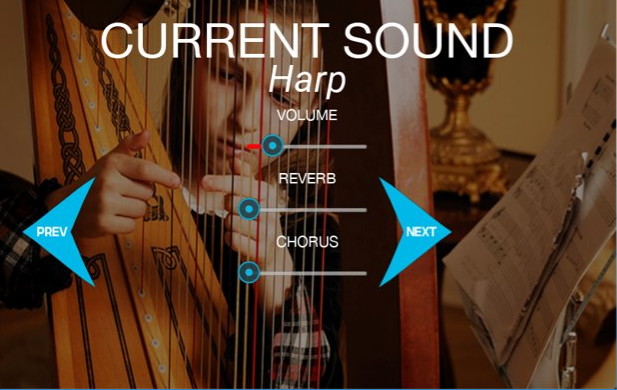
\includegraphics[width=0.90\textwidth]{images/ui.png}
 \caption{Sample User Interface}
\end{figure}



